% !TEX root = jbsilvaThesis.tex

%%%%%%%%%%
%%%%%%%%%%%%%%%%%%%%%%%%%%%%%%%%%%%%%%%%%%%%%%%%%%%%%%%%%%%%%

\chapter{\label{chp:het_nucl}Heterogeneous Nucleation Near the Spinodal}

In Chapter~\ref{chp:pseudo} the value of the pseudospinodal field of a \het\ system with fixed magnetic spins was shown to be changed by an effective field due to    fixed spins. The change of the value of the pseudospinodal field should be reflected in the distribution of the size of the clusters. In this chapter the consequences of the shifted pseudospinodal on the scaling of the clusters is explored in systems with fixed magnetic spins. The consequences of the heterogeneities on the properties of the nucleating droplet will be studied by measuring the stable spin density near the center of the droplet. 

As given in Chapter~\ref{chp:nuc_details} by Eqn.~\eqref{eqn:fisherscaling} the scaling of the clusters depends on the distance to the pseudospinodal $\Delta h$, the critical exponent $\tau$, and the critical exponent $\sigma$. 
\begin{equation}
n_s = \frac{\exp{(-\Delta h s^\sigma)}}{s^{\tau-1}}
\tag{\ref{eqn:fisherscaling}}
\end{equation}%%

The percolation exponents $\tau$ and $\sigma$ are related to the critical exponents $\gamma$ and $\beta$ which define the scaling of thermodynamic quantities such as the susceptibility and the magnetization as given in Eqs.~\eqref{eqn:tau} and \eqref{eqn:sigma}. Systems with a small amount of heterogeneity have been studied, especially for the case of dilution. Previous work by Liu et al.~\cite{kangdilute} has shown that only the  critical exponent $\sigma$ is modified by dilution, and the $\tau$  exponent is unchanged. In Liu et al.'s work it was shown that for a small percentage $x$ of dilution $\sigma$ is modified as
%%
\begin{equation}
\label{eqn:sigmamod}
\sigma(x) = \sigma_0 (1-x)
\end{equation}%%

If there is an unequal number of fixed spins in the stable and metastable directions,  it is necessary to correct the value of $h_s$ for the effective field in Eqn.~\eqref{eq:heter_w_field} as observed in Fig.~\ref{fig:ps_heter_n}. The resulting $\Delta h_s = h_s - h_{\rm applied} - h_{\rm effective}$ and $\sigma = \sigma_0 (1-x)$ will be used in conjunction with the \mf\ critical exponents in Eqn.~\eqref{eqn:fisherscaling}. 

\section{Percolation Mapping and the Critical Nucleation Droplet}
\label{heterpercolation}

After generating a configuration of fixed spins in a given configuration the system was simulated using the Metropolis algorithm to generate spin configurations after the initial transients. Two different possible configuration types (Quilt/Random) as discussed in Chapter~\ref{chp:nuc_details} were generated for the fixed spins. A quilt pattern is the result of putting together patches the size of the interaction range with a given density of fixed spins. The random pattern is generated by choosing the fixed spins with a given set of directions and defining the location by a uniformly randomly generated set of coordinates. Due to the size and nature  of the quilt pattern, it has considerably less \het\ effects compared to the uniformly random fixed spin configuration.

Percolation clusters were then determined for the resulting spin configurations from the dynamic set of stable spins with the bond probability given by Eqn.~\eqref{eqn:bondprob} which we repeat here for convenience. The statistics for the number of clusters was calculated. 
\begin{equation}
	p_b = 1-\exp{[-\beta J(1-\rho_s)]}
	\tag{\ref{eqn:bondprob}}
\end{equation}%%

%%
%%
%%
\begin{figure}[!h]
 \centering
 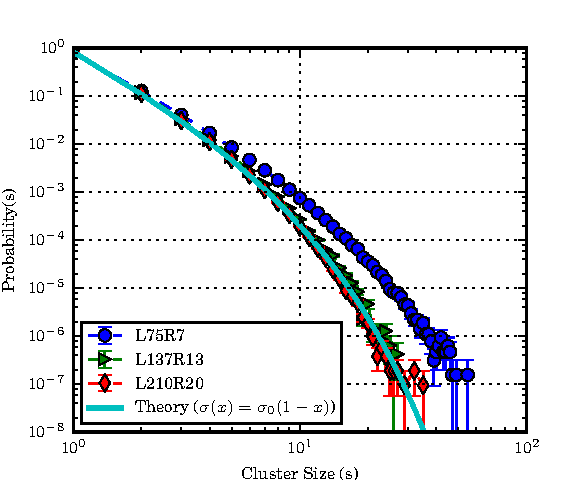
\includegraphics[scale=1.2]{Figures/cluster/percHeter01-quilt_2.pdf}
 \caption{Scaling of the percolation clusters for $T=9T_c/20$ and $h=0.6$ with $5\%$  of spins fixed in the stable directions in a quilt pattern. The distribution $n_s$ is consistent with Eqn.~\eqref{eqn:sigmamod} as the system size increases.
}
 \label{fig:percclusterquilt}
\end{figure}%%
%%
\begin{figure}[!h]
 \centering
 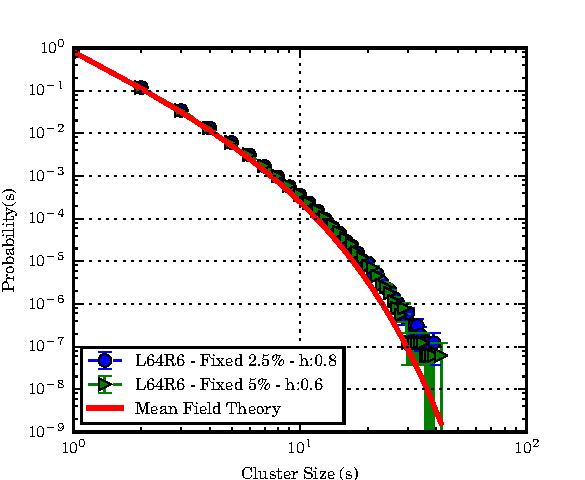
\includegraphics[scale=1.1]{Figures/cluster/percHeter-ranDel.pdf}
 \caption{Cluster size scaling for $T=9T_c/20$, $L=64$, $R=6$, and 5\% spins fixed in the stable directions distributed with uniformly random choice of coordinates. A small deviation due to \het\ effects is observed  compared to Fig.~\ref{fig:percclusterquilt}}
 \label{fig:percclusterheter}
\end{figure}%%

In Fig.~\ref{fig:percclusterquilt} a quilt pattern of 5\% fixed spins in the stable direction was generated for systems of varying size and interaction range  with an approximately equal ratio between the length of the lattice $L$ and $R$ at  field $0.6$. It is observed that the cluster scaling approaches the form in Eqn.~\eqref{eqn:fisherscaling} with the modified exponent given in Eqn.~\eqref{eqn:sigmamod} as $L$ is increased despite the presence of the fixed spins. There is a small deviation as \het\ effects are introduced by using stable fixed spins distributed with an uniformly random choice of coordinates (see Fig.~\ref{fig:percclusterheter}).

\section{Properties of the  Nucleating Droplet}

The properties of the  nucleating droplet are of particular importance in determining both the type of nucleation and the ease of initiating a nucleation event. As discussed, classical nucleation is characterized by a compact droplet with a sharp interface between the stable and metastable phases. Spinodal nucleation has a ramified object of stable spins with a smooth interface between the stable and metastable phase. The density of the stable spins in the \het\ system will be measured to determine if the structure of the nucleating droplet differs from the structure of the droplet in the \homo\ nucleation case.
%%
\begin{figure}[!h]
 \centering
 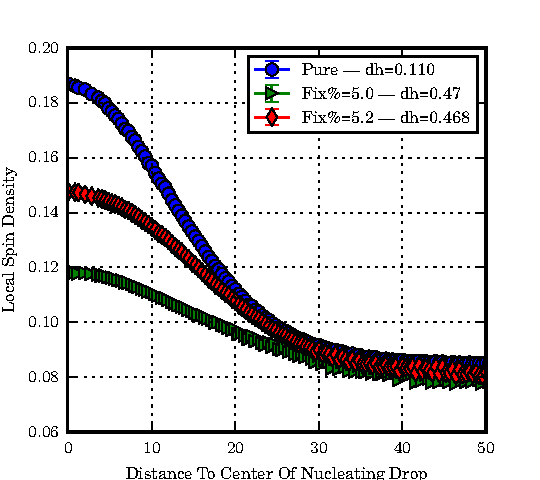
\includegraphics[scale=1.05]{Figures/density/density_fix_spinodal.pdf}
 \caption{The stable spin density as a function of the distance from the center of mass of the nucleating droplet for different values of $\Delta h_s$. Note the sparseness of the \het\ nucleating droplets relative to the density for the \homo\ nucleating droplet. }
 \label{fig:densityfixdh}
\end{figure}%%
%%
\begin{figure}[!h]
 \centering
 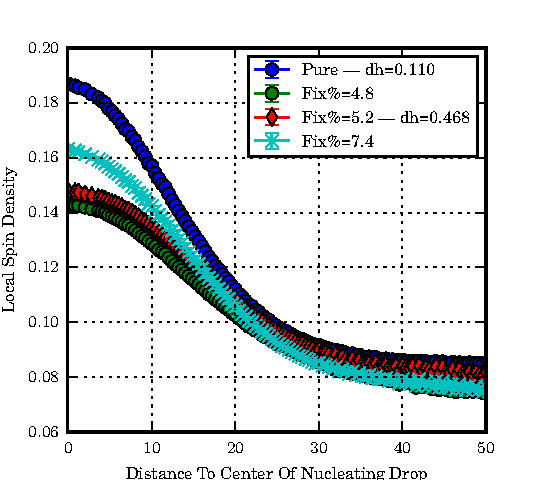
\includegraphics[scale=1.05]{Figures/density/density_fix_var.pdf}
 \caption{ The stable spin density as a function of the distance from the center of mass of the nucleating droplet as in Fig.~\ref{fig:densityfixdh}, but for different amounts of fixed spins. }
 \label{fig:densityfixds}
\end{figure} %%
%%

To measure the stable spin density, the system was simulated with varying amounts of fixed spins to create \het\ nucleation events. To isolate the effects due to the fixed spins $\Delta h_s$ was fixed. Snapshots of the system at the time of nucleation were then gathered for many nucleation events. The location of the nucleating droplet was determined by letting the simulation evolve until the  center of mass of the largest cluster  does not fluctuate. The density of stable spins was calculated as a function of the distance from the center of mass of the nucleating droplet. In Fig.~\ref{fig:densityfixdh} the density of    the stable direction spins in the nucleating droplet are observed to decrease relative to the \nd\ in the \homo\ case. The density of this nucleating droplet should become more ramified as the spinodal is approached. Hence, apart from  any \het\ effects, the \homo\ system is supposed to be the least dense droplet due to its smaller distance to the spinodal field. However, the \het\ system appears to be less dense than the \homo\ system. A possible explanation of the sparseness of the nucleating droplet is  that the fixed spins allow for the crossing of the nucleation barrier by sparser nucleating droplets. %%

This  effect due to the fixed spins   is shown in Fig.~\ref{fig:densityfixds}, where the amount of fixed spins is varied. It is expected from Eqn.~\eqref{eq:heter_w_field} that a larger number of fixed stable spins will increase the likelihood of nucleation occurring. Therefore it is expected that nucleation will occur at the location of the strongest ``effective" field given by the largest grouping of fixed stable spins. In Fig.~\ref{fig:densityfixdens} I observe the coincidence between the locations of the largest stable effective field location and the location of the nucleating droplet. %%
%%
\begin{figure}[!h]
 \centering
 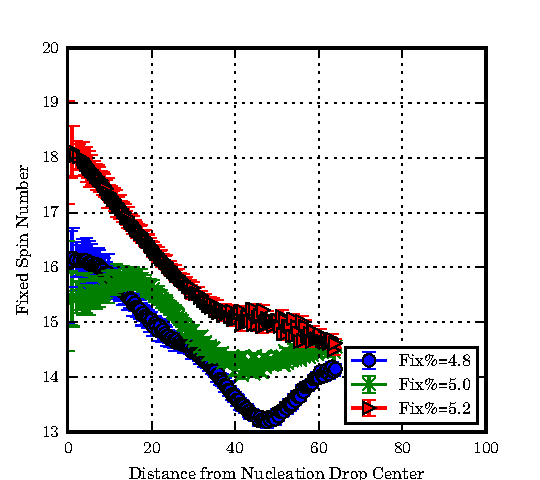
\includegraphics[scale=1.05]{Figures/density/density_fix_density_all.pdf}
 \caption{The number of fixed spins in the stable direction versus the distance from the center of mass of the nucleating droplet.  As expected, nucleation occurs near the maxima of the number of stable fixed spins. }
 \label{fig:densityfixdens}
\end{figure}%%

